\documentclass[tikz,border=10pt]{standalone}
\usepackage{tikz}
\usetikzlibrary{arrows.meta, positioning, fit}

\begin{document}

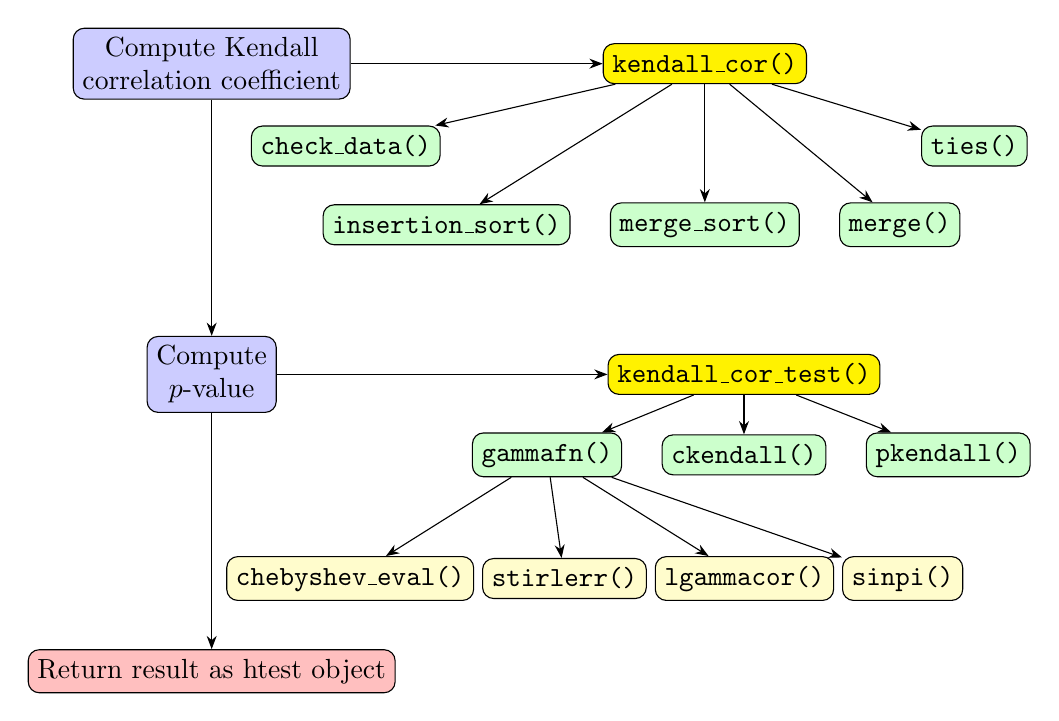
\begin{tikzpicture}[
  node distance=1.5cm and 2.5cm,
  every node/.style={draw, rounded corners, align=center},
  process/.style={fill=blue!20},
  function/.style={fill=green!20},
  helper/.style={fill=yellow!20},
  arrow/.style={-{Stealth}}
]

% Main steps in kendall_cor_test
\node[process] (compute_tau) {Compute Kendall\\correlation coefficient};
\node[process, below=of compute_tau, yshift=-1.5cm] (compute_pvalue) {Compute\\$p$-value};
\node[process, below=of compute_pvalue, yshift=-1.5cm, fill = pink] (return_result) {Return result as htest object};

% Functions called by kendall_cor_test
\node[function, right=of compute_tau, xshift=0.7cm, fill = yellow] (kendall_cor_func) {\texttt{kendall\_cor()}};
\node[function, right=of compute_pvalue, xshift=1.7cm, fill = yellow] (kendall_cor_test_func) {\texttt{kendall\_cor\_test()}};

% Functions called by kendall_cor_
\node[function, below=of kendall_cor_func] (merge_sort) {\texttt{merge\_sort()}};
\node[function, left=of merge_sort, xshift=2cm] (insertion_sort) {\texttt{insertion\_sort()}};
\node[function, left=of insertion_sort, xshift=4cm, yshift=1cm] (check_data) {\texttt{check\_data()}};
\node[function, right=of merge_sort, xshift=-2cm] (merge) {\texttt{merge()}};
\node[function, right=of merge, xshift=-3cm, yshift=1cm] (ties) {\texttt{ties()}};

% Functions called by pkendall_
\node[function, below=of kendall_cor_test_func, yshift=1cm] (ckendall) {\texttt{ckendall()}};
\node[function, left=of ckendall, xshift=2cm] (gammafn) {\texttt{gammafn()}};
\node[function, right=of ckendall, xshift=-2cm] (pkendall) {\texttt{pkendall()}};

% Functions called by gammafn_
\node[helper, below=of gammafn, xshift=-2.5cm, yshift=0.5cm] (chebyshev_eval) {\texttt{chebyshev\_eval()}};
\node[helper, right=of chebyshev_eval, xshift=-2.4cm] (stirlerr) {\texttt{stirlerr()}};
\node[helper, right=of stirlerr, xshift=-2.4cm] (lgammacor) {\texttt{lgammacor()}};
\node[helper, right=of lgammacor, xshift=-2.4cm] (sinpi) {\texttt{sinpi()}};

% Arrows
\draw[arrow] (kendall_cor_func) -- (check_data);
\draw[arrow] (compute_tau) -- (compute_pvalue);
\draw[arrow] (compute_pvalue) -- (return_result);

\draw[arrow] (compute_tau) -- (kendall_cor_func);
\draw[arrow] (compute_pvalue) -- (kendall_cor_test_func);

\draw[arrow] (kendall_cor_func) -- (insertion_sort);
\draw[arrow] (kendall_cor_func) -- (merge_sort);
\draw[arrow] (kendall_cor_func) -- (merge);
\draw[arrow] (kendall_cor_func) -- (ties);

\draw[arrow] (kendall_cor_test_func) -- (ckendall);
\draw[arrow] (kendall_cor_test_func) -- (pkendall);
\draw[arrow] (kendall_cor_test_func) -- (gammafn);

\draw[arrow] (gammafn) -- (chebyshev_eval);
\draw[arrow] (gammafn) -- (stirlerr);
\draw[arrow] (gammafn) -- (lgammacor);
\draw[arrow] (gammafn) -- (sinpi);

\end{tikzpicture}

\end{document}
